\documentclass{beamer}
\usepackage[font={footnotesize,it}]{caption}
\usepackage[utf8]{inputenc}
\usepackage[english]{babel}
%\usepackage{amsmath,amssymb}
\usepackage{csvsimple}
\usepackage{tikz}
\usepackage{pgfplots}
%\usepackage{float}
\pgfplotsset{compat=1.14}
%\usepackage{xcolor}
\usepackage{graphicx}
\usepackage[textsize=tiny]{todonotes}


\usepackage{pgfplotstable}

\newcommand{\chartheight}{7cm}
\newcommand{\chartlegendpos}{(0.5,-0.2)}

\definecolor{cGas}{RGB}{202,178,214}
\definecolor{cCoal}{RGB}{180,180,180}
\definecolor{cNuclear}{RGB}{253,191,111}
\definecolor{cWind}{RGB}{178,223,138}
\definecolor{cHydro}{RGB}{166,206,227}
\definecolor{cInterconnect}{RGB}{251,154,153}


%
% GENERATION SCHEDULE
%

\newcommand{\chartgenschedstacked}[1]{%
    \pgfplotstableread[col sep=comma]{#1}\loadedtable
    \begin{tikzpicture}
        \begin{axis}[
            ymin=0,
            minor tick num=4,
            enlarge x limits=false,
            const plot,
            axis on top,
            stack plots=y,
            cycle multi list={%
                {cWind!60!black,fill=cWind},%
                {cNuclear!60!black,fill=cNuclear},%
                {cGas!60!black,fill=cGas},%
                {cCoal!60!black,fill=cCoal},%
                {cInterconnect!60!black,fill=cInterconnect},%
                {cHydro!60!black,fill=cHydro},%
             },
            xlabel={Time (h)},
            ylabel={Generation (GW)},
            width=\columnwidth,
            height=\chartheight,
            legend style={
                area legend,
                at={\chartlegendpos},
                anchor=north,
                legend columns=3}
            ]

        \addplot table[x=StartTime,y expr=\thisrow{Wind} * 0.001] from \loadedtable \closedcycle;
        \addplot table[x=StartTime,y expr=\thisrow{Nuclear} * 0.001] from \loadedtable \closedcycle;
        \addplot table[x=StartTime,y expr=\thisrow{Gas} * 0.001] from \loadedtable \closedcycle;
        \addplot table[x=StartTime,y expr=\thisrow{Coal} * 0.001] from \loadedtable \closedcycle;
        \addplot table[x=StartTime,y expr=\thisrow{Interconnect} * 0.001] from \loadedtable \closedcycle;
        \addplot table[x=StartTime,y expr=\thisrow{Hydro} * 0.001] from \loadedtable \closedcycle;
        \legend{Wind, Nuclear, Gas, Coal, Intercon., Hydro}
        \end{axis}
    \end{tikzpicture}%
}


%
% CO2 RAMPDOWN
%

\newcommand{\chartrampdown}{%
\pgfplotstableread[col sep=comma]{output/co2rampdown.csv}\loadedtable
\begin{tikzpicture}

	\begin{axis}[
        width=0.9\columnwidth,
        height=\chartheight,
		ybar stacked,
		axis y line*=left,
		ylabel={Daily Output (GWh)},
		xlabel={Reduction in CO2 Emissions Limit (\%)},
        ymin=0,
        legend style={
          area legend,
          at={\chartlegendpos},
          anchor=north,
          legend columns=3}
	]
	\addplot[cWind!60!black,fill=cWind] table[x=Reduction,y expr=\thisrow{Wind}/1000]{\loadedtable};
	\addplot[cNuclear!60!black,fill=cNuclear] table[x=Reduction,y expr=\thisrow{Nuclear}/1000]{\loadedtable};
	\addplot[cGas!60!black,fill=cGas] table[x=Reduction,y expr=\thisrow{Gas}/1000]{\loadedtable};
	\addplot[cHydro!60!black,fill=cHydro] table[x=Reduction,y expr=\thisrow{Hydro}/1000]{\loadedtable};
	\addplot[cCoal!60!black,fill=cCoal] table[x=Reduction,y expr=\thisrow{Coal}/1000]{\loadedtable};
	\addplot[cInterconnect!60!black,fill=cInterconnect] table[x=Reduction,y expr=\thisrow{Interconnect}/1000]{\loadedtable};
        \legend{Wind, Nuclear, Gas, Hydro, Coal, Intercon.}
   \end{axis}

	\begin{axis}[
        width=0.9\columnwidth,
        height=\chartheight,
		axis y line*=right,  
		axis x line = none,
		ylabel={Profit (\textsterling m)}]
			\addplot table[x=Reduction,y expr=\thisrow{Profit}] from \loadedtable;
	\end{axis}  

	\end{tikzpicture}
}


%
% CO2 CREDIT
%

\newcommand{\chartcredit}[1]{%
\pgfplotstableread[col sep=comma]{#1}\loadedtable
\begin{tikzpicture}

	\begin{axis}[
        width=0.9\columnwidth,
        height=\chartheight,
		ybar stacked,
		axis y line*=left,
		xlabel={Carbon Price (\textsterling)},
		ylabel={Daily Output (GWh)},
        bar width=4pt,
        xmin=-5,
        xmax=105,
        ymin=0,
        legend style={
          area legend,
          at={(0.5,-0.2)},
          anchor=north,
          legend columns=3}
	]
	\addplot[cWind!60!black,fill=cWind] table[x=Co2Price,y expr=\thisrow{Wind}/1000]{\loadedtable};
	\addplot[cNuclear!60!black,fill=cNuclear] table[x=Co2Price,y expr=\thisrow{Nuclear}/1000]{\loadedtable};
	\addplot[cGas!60!black,fill=cGas] table[x=Co2Price,y expr=\thisrow{Gas}/1000]{\loadedtable};
	\addplot[cCoal!60!black,fill=cCoal] table[x=Co2Price,y expr=\thisrow{Coal}/1000]{\loadedtable};
	\addplot[cHydro!60!black,fill=cHydro] table[x=Co2Price,y expr=\thisrow{Hydro}/1000]{\loadedtable};
	\addplot[cInterconnect!60!black,fill=cInterconnect] table[x=Co2Price,y expr=\thisrow{Interconnect}/1000]{\loadedtable};
        \legend{Wind, Nuclear, Gas, Coal, Hydro, Intercon.}
   \end{axis}

	\begin{axis}[
        width=0.9\columnwidth,
        height=\chartheight,
		axis y line*=right,  
		axis x line = none,
        xmin=-5,
        xmax=105,
		ylabel={Profit (\textsterling m)}
		]
			\addplot table[x=Co2Price,y expr=\thisrow{Profit}/1000000] from \loadedtable;
	\end{axis}  

	\end{tikzpicture}
}


%
% CARBON TAX
%

\newcommand{\chartcarbontax}[1]{%
\pgfplotstableread[col sep=comma]{#1}\loadedtable
\begin{tikzpicture}

	\begin{axis}[
        width=0.9\columnwidth,
        height=\chartheight,
		ybar stacked,
		axis y line*=left,
		xlabel={Carbon Tax (\textsterling)},
		ylabel={Daily Output (GWh)},
        bar width=4pt,
        xmin=-5,
        xmax=105,
        ymin=0,
        legend style={
          area legend,
          at={(0.5,-0.2)},
          anchor=north,
          legend columns=3}
	]
	\addplot[cWind!60!black,fill=cWind] table[x=Co2Price,y expr=\thisrow{Wind}/1000]{\loadedtable};
	\addplot[cNuclear!60!black,fill=cNuclear] table[x=Co2Price,y expr=\thisrow{Nuclear}/1000]{\loadedtable};
	\addplot[cGas!60!black,fill=cGas] table[x=Co2Price,y expr=\thisrow{Gas}/1000]{\loadedtable};
	\addplot[cCoal!60!black,fill=cCoal] table[x=Co2Price,y expr=\thisrow{Coal}/1000]{\loadedtable};
	\addplot[cHydro!60!black,fill=cHydro] table[x=Co2Price,y expr=\thisrow{Hydro}/1000]{\loadedtable};
	\addplot[cInterconnect!60!black,fill=cInterconnect] table[x=Co2Price,y expr=\thisrow{Interconnect}/1000]{\loadedtable};
        \legend{Wind, Nuclear, Gas, Coal, Hydro, Intercon.}
   \end{axis}

	\begin{axis}[
        width=0.9\columnwidth,
        height=\chartheight,
		axis y line*=right,  
		axis x line = none,
        xmin=-5,
        xmax=105,
		ylabel={Profit (\textsterling m)}
		]
			\addplot table[x=Co2Price,y expr=\thisrow{Profit}/1000000] from \loadedtable;
	\end{axis}  

	\end{tikzpicture}
}




%
% GEN SCHEDULE TABLE
%


\newcommand{\productiontable}[1]{%
    \begin{tabular}{lcccccc}
		\hline
		\textbf{Period} & \textbf{Gas} & \textbf{Coal} & \textbf{Nuclear} & \textbf{Wind} & \textbf{Hydro} & \textbf{Interconnect} \\ \hline
		\csvreader[head to column names]{#1}{}
		{\Period & \Gas & \Coal & \Nuclear & \Wind & \Hydro & \Interconnect \\} \\ \hline
    \end{tabular}
}




%%%%%%%%%%%%%%%%%%%%%%%%%%%%%%%%%%%%%%%%%%%%%%%%%%%%%%%%%%%%%%%%%%%%%%%%
%%%%%%%%%%%%%%%%%%%%%%%%%%%%%%%%%%%%%%%%%%%%%%%%%%%%%%%%%%%%%%%%%%%%%%%%
%%%%%%%%%%%%%%%%%%%%%%%%%%%%%%%%%%%%%%%%%%%%%%%%%%%%%%%%%%%%%%%%%%%%%%%%






\newcommand{\chartgencarbonprice}[2]{%
    \pgfplotstableread[col sep=comma]{#2}\loadedtable
    \begin{tikzpicture}
        \begin{axis}[
        	title={#1},
            ymin=0,
            minor tick num=4,
            enlarge x limits=false,
            const plot,
            axis on top,
            stack plots=y,
            cycle multi list={%
                {cGas!60!black,fill=cGas},%
                {cCoal!60!black,fill=cCoal},%
                {cNuclear!60!black,fill=cNuclear},%
                {cWind!60!black,fill=cWind},%
                {cHydro!60!black,fill=cHydro},%
                {cInterconnect!60!black,fill=cInterconnect},%
             },
            xlabel={Time (h)},
            ylabel={Generation (MW)},
            width=\columnwidth,
            height=7cm,
            legend style={
                area legend,
                at={(0.5,-0.2)},
                anchor=north,
                legend columns=3}
            ]

        \addplot table[x=StartTime,y=Gas] from \loadedtable \closedcycle;
        \addplot table[x=StartTime,y=Nuclear] from \loadedtable \closedcycle;
        \addplot table[x=StartTime,y=Coal] from \loadedtable \closedcycle;
        \addplot table[x=StartTime,y=Wind] from \loadedtable \closedcycle;
        \addplot table[x=StartTime,y=Hydro] from \loadedtable \closedcycle;
        \addplot table[x=StartTime,y=Interconnect] from \loadedtable \closedcycle;
        %\addplot+[stack plots=false] table[x=time,y=memtotal]     from \loadedtable;
        \legend{Gas, Coal, Nuclear, Wind, Hydro, Interconnect}
        \end{axis}
	\end{axis}  
    
    \end{tikzpicture}%
}



%############################################################
% Here is Matthew's very badly done graph of Hydro, Pump, and Reserve
% #####

% Color theme
\definecolor{cHydroReserve}{RGB}{253,191,111}
\definecolor{cPump}{RGB}{178,223,138}
\definecolor{cHydro}{RGB}{166,206,227}

\pgfplotsset{
    ylabel right/.style={
        after end axis/.append code={
            \node [rotate=90, anchor=north] at (rel axis cs:1,0.5) {#1};
        }   
    }
}


\newcommand{\charthydro}[1]{%
    \pgfplotstableread[col sep=comma]{#1}\loadedtable
    \begin{tikzpicture}
        \begin{axis}[
            ymin=0,
            minor tick num=4,
            enlarge x limits=false,
            const plot,
            axis on top,
            xlabel={Time (h)},
            ylabel={Power (GW)},
            width=\columnwidth,
            height=7cm,
            ylabel right=Energy (GWh),
            legend style={
                at={(0.5,-0.2)},
                anchor=north,
                legend columns=3}
            ]

        \addplot table[x=StartTime,y expr = \thisrow{Hydro} * 0.001] from \loadedtable;
        \addplot table[x=StartTime,y expr = \thisrow{Pump} * 0.001] from \loadedtable;
        %\addplot table[x=StartTime,y=HydroReserve] from \loadedtable; % old reservoir level plot
        % new reservoir level plot
        \addplot[
    sharp plot,
    mark = square*,
    ]
    coordinates {
    (0,0.800)(6,12.800)(8,13.600)(16,9.600)(20,3.200)(22,0)(24,0.800)
    };
        %\addplot+[stack plots=false] table[x=time,y=memtotal]     from \loadedtable;
        \legend{Discharge, Pump, Reserve Level}
        \end{axis}
            
    \end{tikzpicture}%
}
% #######################
% End of badly done graph
% #######################



% Hydro table Matthew
\newcommand{\hydrotable}[1]{%
    \begin{tabular}{lccc}
		\hline
		\textbf{Period} & \textbf{Hydro} & \textbf{Pump} &\textbf{Reserve}
        \\ \hline
		\csvreader[head to column names]{#1}{}
		{\Period & \Hydro & \Pump & \HydroReserve \\} \\ \hline
    \end{tabular}
}


\author{Mark Alexander, Abby Li,\texorpdfstring{\\}{}Szymon Sacher, and Matthew Yau}
\date{April 2017}

%\setbeameroption{show notes}

% Custom chart settings for presentation only
\renewcommand{\chartheight}{5.5cm}
\renewcommand{\chartlegendpos}{(0.5,-0.3)}

% Presentation theme/color/etc
\mode<presentation>
{
    \usetheme{default}
    \usecolortheme{orchid}
    \setbeamertemplate{navigation symbols}{}
    \setbeamertemplate{caption}[numbered]
}

% Details
\title[EPower Case Study]{\Huge EPower\\[0.2cm]\large Case Study}

\institute{LPMS Consultancy}

\begin{document}
	
    % ################################################
    %  TITLE, INTRO AND BASE CASE [MATTHEW]
    % ################################################
    
    %
    % TITLE PAGE
    %
    
    \begin{frame}
    	\titlepage
    \end{frame}
    
    %
    % OVERVIEW
    %
    
    \begin{frame}{Topic Overview}
        
        \tableofcontents
            
    \end{frame}
    
    %
    % CURRENT OPERATIONS - OVERVIEW
    %
    
    \section{Current Operations}
    
    \begin{frame}{Current Operations - Overview}
    	\begin{itemize}
    	\item Objective: maximize profit
        \item Decisions: Generate, Pump, Hydro reserve, Increase 
        \item Considerations: demand, max output, costs, emissions limits, price of electricity
        \item Optimal: total daily profit of £2 million
        	\begin{itemize}
                \item Revenue: £15 million
                \item Running cost: £13 million
                \item Increase cost: £0.4 million
        	\end{itemize}
    	\end{itemize}
    \end{frame}
    
    %
    % CURRENT OPERATIONS - GENERATION SCHEDULE
    %
    
    \begin{frame}{Current Operations - Generation Schedule}
    
    	\begin{figure}[H]
            \centering
            \chartgenschedstacked{output/base.csv}
        \end{figure}%

    \end{frame}
    
    %
    % CURRENT OPERATIONS - OBSERVATIONS
    %
    
    \begin{frame}{Current Operations - Observations}
    	\begin{itemize}
            \item Wind power always operates at average max output
            \item Hydro fully used during evening
            \item Pump during quiet hours
            \item Constant nuclear usage
            \item No interconnect usage        
    	\end{itemize}
    \end{frame}
    
    %
    % CURRENT OPERATIONS - HYDRO ACTIVITY
    %
    
    \begin{frame}{Current Operations - Hydro Activity}
    	    	
    	\begin{figure}[H]
            \centering
            \charthydro{output/base.csv}
        \end{figure}
    
    \end{frame}
    

    % ################################################
    %  DAILY MULTIPLIERS [ABBY]
    % ################################################
    
    \section{Preparing for Uncertainty}
    
    %
    % EFFECTS
    %
    
    \begin{frame}{20\% Increase in Demand and Wind - Effects}
    
        \begin{figure}[H]
            \centering
            \chartgenschedstacked{output/multipliers.csv}
        \end{figure}
        
        \note[item]{Primary change is that we now need to make use of the interconnect to deal with peak demand.}
        
        \note[item]{This rapidly eats into profit because the interconnect is (the most) expensive sources.}
    
    \end{frame}
    
    %
    % STRATEGIES
    %
    
    \begin{frame}{20\% Increase in Demand and Wind - Strategies}
        
        \begin{itemize}
        
            \item  \textbf{Flatten out demand} throughout the day, e.g. \textbf{offering incentives} to consume during off-peak hours.
            	
                \begin{itemize}
            
            		\item Large/industrial customers: build relationships and negotiate agreements.
            
            		\item Domestic customers: \textbf{introduce differential tariffs}.
            
                \end{itemize}
            
            \item \textbf{Increase maximum hydro output} if viable.
            
            	\begin{itemize}
                	
                    \item Hydro reservoir serves a similar overflow function as the interconnect but is much cheaper.
                    
                    \item Here, between 1600 and 2000, hydro is being fully utilized and the marginal value of additional capacity is \textsterling 45.
                    
                \end{itemize}   
            
        \end{itemize}
    
    \end{frame}
    
    %
    % GENERALIZATION
    %
	
    \begin{frame}{Variable Demand and Wind - Generalization}
    	
        	\begin{itemize}

                \item Optimal strategy will vary by multiplier value.  Hard to decide general optimal policy given only one of them.

                \item  Better approach: \textbf{simulate effect on profit} using \textit{distributions} of wind and demand inputs \note[item]{ to obtain a generalized optimal policy}.

                \item Best approach: \textbf{adapt dynamically to changing conditions} throughout the day.  May not be suitable for some sources.  \note[item]{Not all sources can adapt dynamically.  How to decide nuclear output is critical.}

			\end{itemize}   
    
    \end{frame}

    
    % ################################################
    %  REDUCED CO2 - INVESTING IN ADDITIONAL CAPACITY [MARK]
    % ################################################
    
    \section{Planning for CO\texorpdfstring{\textsubscript{2}}{2} Reduction}
    
    \subsection{Investing in Additional Capacity}
    
        \begin{frame}{Reduced CO\textsubscript{2} Limits - Current Setup}
    
       	\chartrampdown
        
    \end{frame}
    
    \begin{frame}{Reduced CO\textsubscript{2} Limits - Current Setup}
    
        \begin{itemize}
    
    		\item Scenario: CO\textsubscript{2} emissions limits are reduced by 50\%.
                
                \pause
    	
        	\item If the new CO\textsubscript{2} limits were introduced today:
    
            \begin{itemize}

                \item A daily \textbf{loss} of \textsterling 2.5 million would be incurred.

                \item Unlike the previous case, this loss occurs on what is considered to be the \textit{average} day.  Long-term losses would likely be extensive.

            \end{itemize}
         
         \end{itemize}
        
    \end{frame}
      
        % Coal is completely eliminated.  Coal is currently the prime cheap energy source, but it's just too carbon-heavy to have a place in this reduced carbon schedule.  This pushes up costs.
        
        % Again use of the interconnect, which is expensive.  But in this case as said it's being used on the average day, which is much more of a problem than using it as a rare overflow safety feature.
        
    
    %
    % 1 GW INVESTMENT
    %
    
    \begin{frame}{Reduced CO\textsubscript{2} Limits - Investing in Output Capacity}
    
        Proposal: invest in 1 GW of extra capacity for one source.
        
        	\pause
    
              \begin{itemize}

                  \item The best outcome arises from adding the 1 GW to wind capacity, closely followed by nuclear.
                  
                  \pause

                  \item In either case, losses are approximately halved to \textsterling 1.4 million.
                  
                  \pause

                  \item \note[item]{But this is still a loss.}  In fact, \textbf{there is no investment of 1 GW that will result in a return to profit}, let alone achieve current profit levels.

              \end{itemize}
        
    \end{frame}
    
    %
    % GENERALIZED INVESTMENT
    %
    
    \begin{frame}{Reduced CO\textsubscript{2} Limits - Investing in Output Capacity}

              
               Further analysis:
              
                \begin{itemize}

                      \item A greater increase in capacity is required, but where and how much?  Our analysis shows:
                      
                      \pause
                      
                        \item A 2.5 GW investment in either wind or nuclear output capacity would return operations to a small profit of approximately \textsterling 200,000-300,000.

\item However, this trend does not continue for both.

	\pause

\item \textbf{A 4 GW expansion of wind capacity would restore profit to current levels}.

\item A 4 GW expansion of Nuclear will not yield the same outcome, due to the increased running costs of nuclear power.

%\item Investment in the capacity of other sources is not generally worthwhile.

                \end{itemize}
        
    \end{frame}
    
    
    
    % ################################################
    %  REDUCED CO2 - EMISSIONS MARKET [SZYMON]
    % ################################################
    
    \subsection{Emissions Market Schemes and Carbon Tax}
    
    %
    % CARBON CREDITS MARKET
    %
    
  \begin{frame}{Carbon Credits Market}
  
 EPower will be allocated 100000 units of CO\textsubscript{2} emission:
      \small
        \begin{itemize}
            \item Fair price of carbon dioxide: £60

            \item EPower can propose introducing offsetting actions in exchange for higher emissions limit 
            \item Use carbon credits market
        \end{itemize}      
    
%    	\todo[inline,caption={}]{\textbf{Julian:} Make this chart larger--ditch the caption if necessary.}
        
%         \begin{figure}
%         \centering
%         \footnotesize
%         Expected profit and optimal production schedule
%         	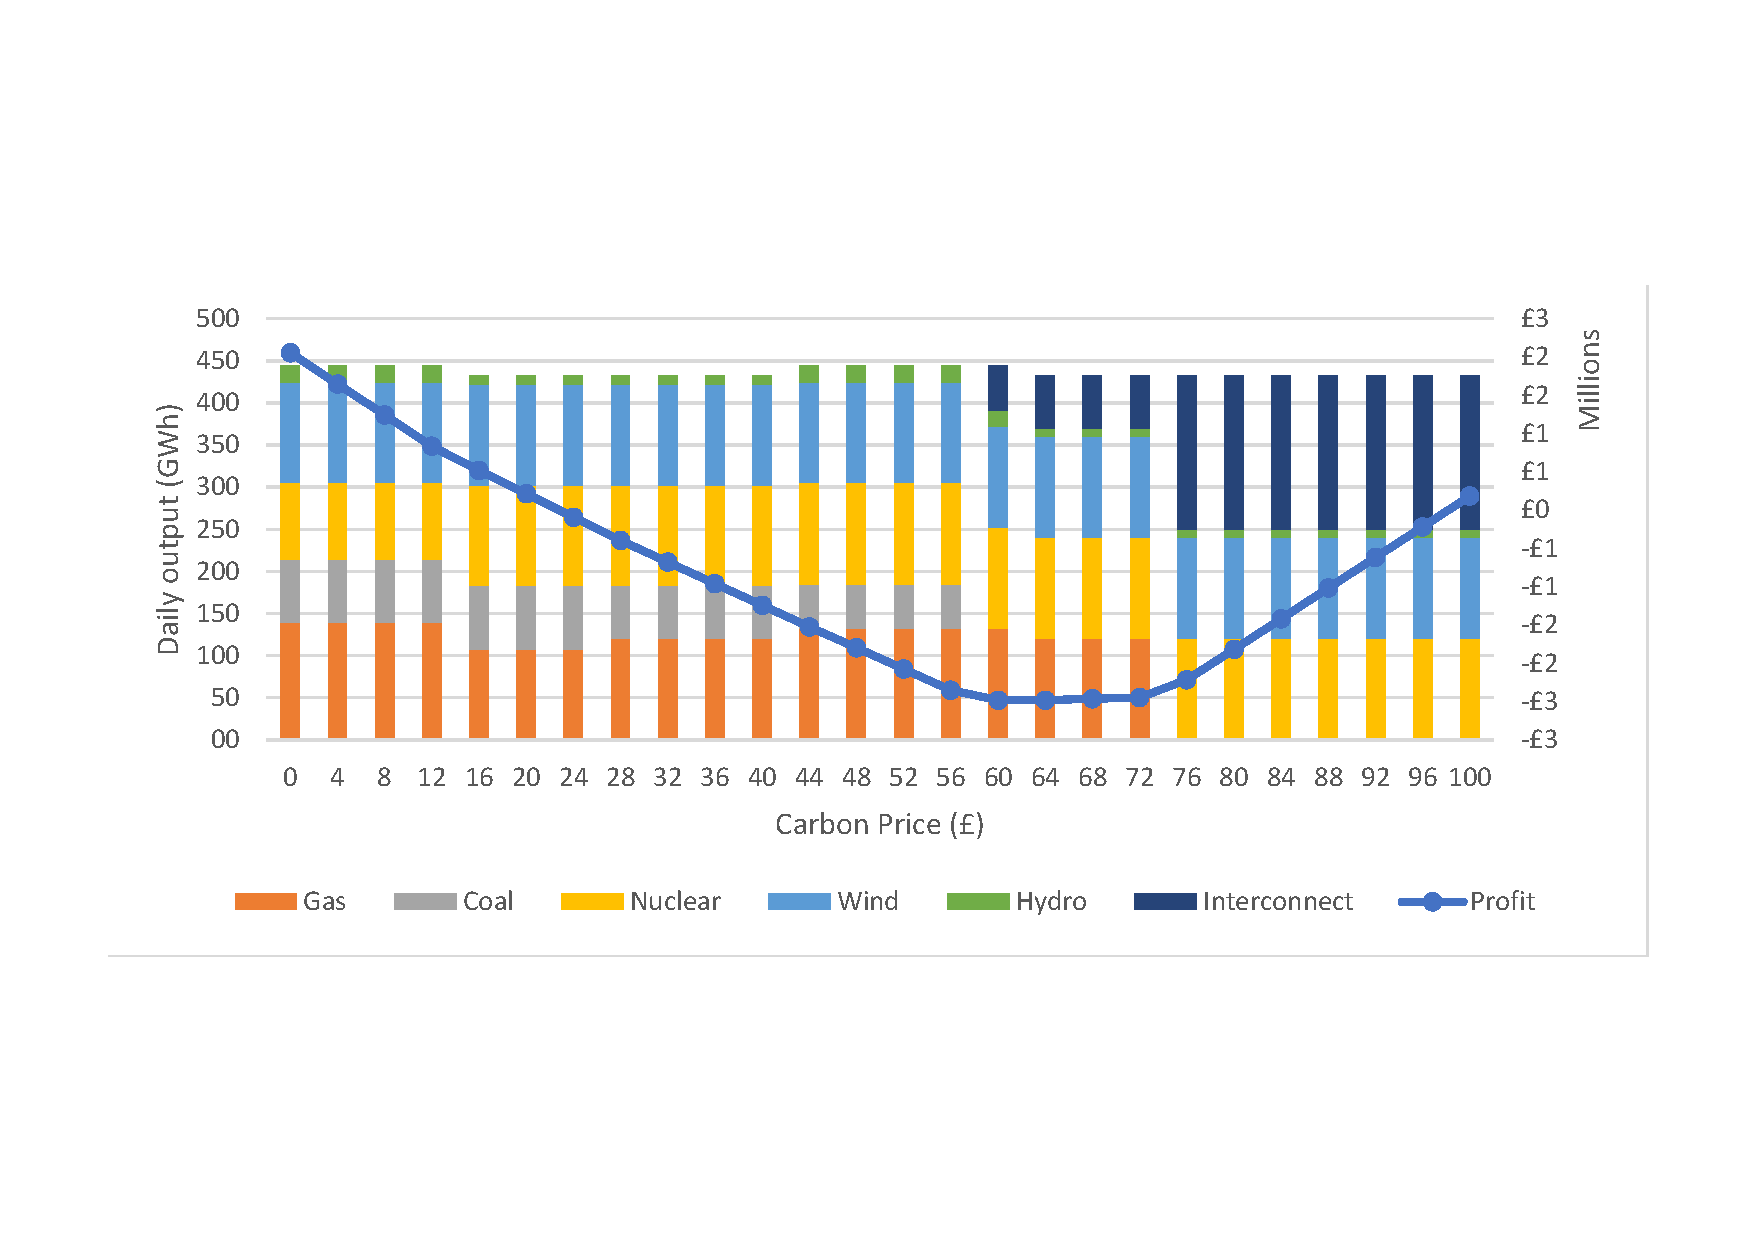
\includegraphics[width=\textwidth]{Graphs/carbon_credit.pdf}

%         \end{figure}
        
        \renewcommand{\chartheight}{4.5cm}
             \begin{figure}
            	\centering
                \chartcredit{output/carbon_credit_full.csv}
            \end{figure}
               
        
    \end{frame}
        
    %
    % CARBON TAX
    %
    
   	\begin{frame}{Carbon Tax}    
    
%    	\todo[inline,caption={}]{\textbf{Mark:} motivate this by saying the considerations are largely similar to the scenarios being considered?  Essentially "there is another CO2-related scenario on the horizon.  Incorporating this into the current considerations will provide a better longer term/more durable strategy, etc."  No use them devising a policy for reduced CO2 (and investing tons of capital into particular sources) if it's not also at least reasonably compatible with the Paris Agreement changes which will come down the pipeline.}

        In light of Paris Agreement, EPower should prepare for ``carbon tax". Following are likely to be impacted: 
        \small
            \begin{itemize}
            \item Market price of electricity
            \item Electricity demand
            \item Running cost of interconnect
            \end{itemize}


%              \begin{figure}
%              \footnotesize Expected profit and optimal production schedule
%             \centering
%                 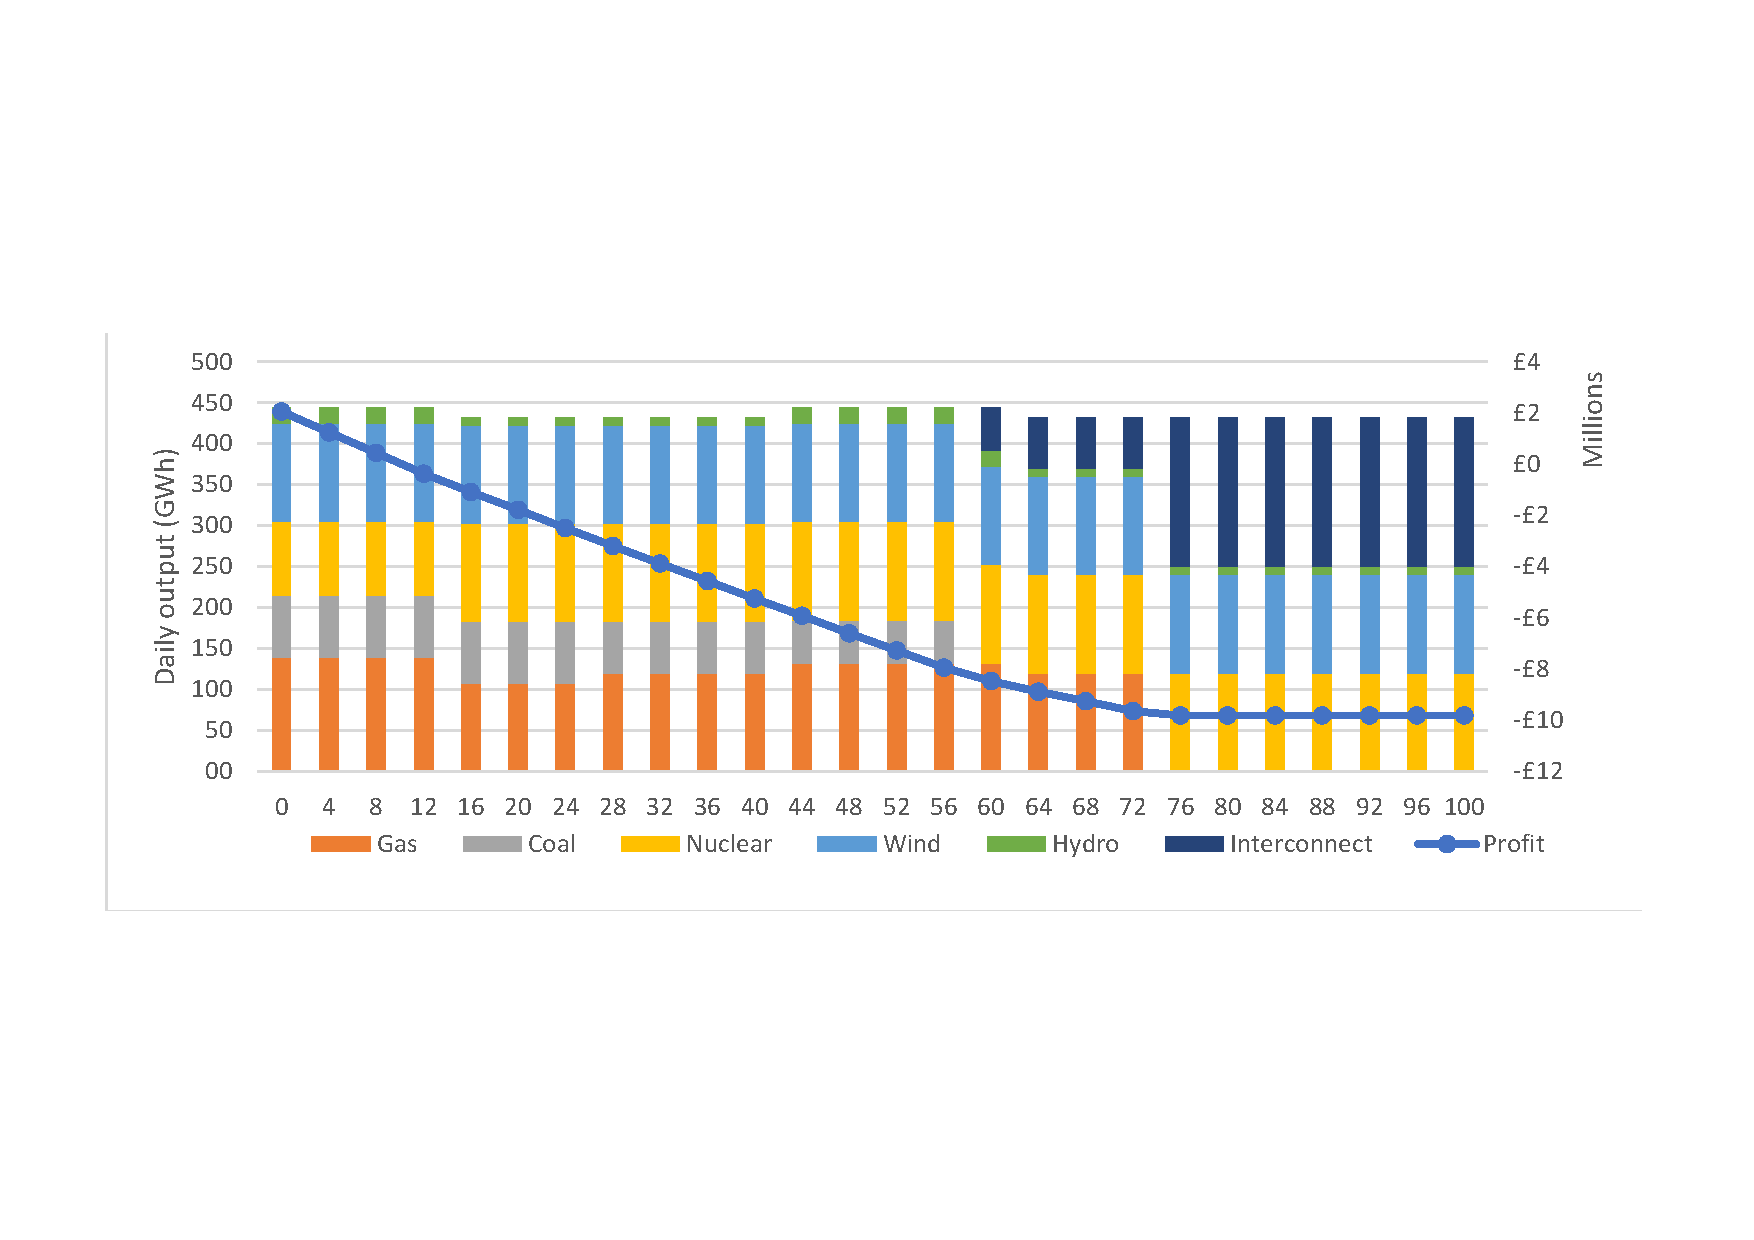
\includegraphics[width=\textwidth]{Graphs/carbon_tax.pdf}
                
%             \end{figure}
            
            \renewcommand{\chartheight}{4.5cm}
             \begin{figure}
            	\centering
                \chartcarbontax{output/carbon_tax_full.csv}
            \end{figure}
        
    \end{frame}
    
    
  
    
    % ################################################
    %  SUMMARY OF RECOMMENDATIONS [ABBY]
    % ################################################

	\section{Summary of Recommendations}
    
    %
    % SUMMARY
    %
    
    \begin{frame}{Summary of Recommendations}
    
    	\begin{itemize}
        
        	\item Dealing with variable demand and wind availability:

                \begin{itemize}

                    \item Reduce variability of demand throughout the day using incentives for consumers.

                    \item Invest in additional capacity to reduce reliance on expensive sources:
                    
                    \begin{itemize}
                    	
                        \item Wind capacity is most valuable.
                        
                        \item Hydro output may also be worthwhile.
                        
                    \end{itemize}

                \end{itemize}
        
        	\item Reduced CO\textsubscript{2} limits:

                \begin{itemize}

                    \item Add approximately 4000 MW to wind power max capacity
                    
                    \item Other considerations: emission credits market, carbon tax.  Technology to clean the output of `dirty' and cheap sources like coal.

                \end{itemize}
        
        	\item Key takeaway: \textbf{a significant investment in wind capacity would be beneficial} in both scenarios considered.
        
        \end{itemize}
        
    \end{frame}
    
    
        
\end{document}
